\lecture{1}{17. Marts 2026}{Introduction}

\section{Course Information}
These are the personal notes, written by Noah R. B. Hansen for the course in Control Theory at Aarhus University taught by Xuping Zhang, PhD. as part of the BSc in Mechanical Engineering. 

\section{Basic concepts and introduction of control theory}

\begin{definition}[Control System]
  A \textit{control system} is a device, or a set of devices, that manages, commands, directs, or regulates the behavior (output) of other device(s)/system(s)/processes by adjusting the input.
  For an example of a control system refer to the bottom of \Cref{fig:consysex}
\end{definition}

\begin{figure} [ht]
  \centering
  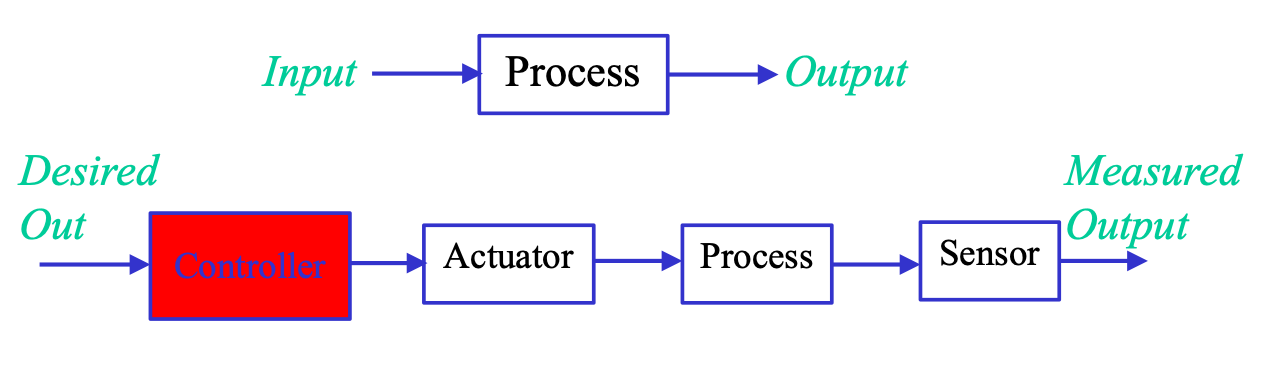
\includegraphics[width=0.8\linewidth]{./figures/consysex.png}
  \caption{Comparison of a simple uncontrolled process and an example control system.}
  \label{fig:consysex}
\end{figure}

In \Cref{fig:consysex} two systems are shown.
The top figure is an uncontrolled process that receives an input and outputs something without concern for anything other than how it is initially set up.

In the bottom diagram, the process is part of a control system.
Here the desired output is fed to a controller that determines what action should be taken to match the real output to the desired one.
The system is then fed to an actuator that applies the commands of the controller to the system, e.g. a motor, valve, heater, pump, brake, etc.
The system is then fed to the process that is being controlled.
This gives a signal to a sensor measuring the state of the process, e.g. a thermometer, encoder, tachometer, barometer, etc.
The output of this sensor is then (ideally) the actual output of the system. 

When talking about control systems we often differentiate between open-loop and closed-loop control systems.

\begin{definition}[Open-loop Control System]
  An open-loop control system utilizes an actuating device to control the process directly without using feedback.
  An example of this is shown on \Cref{fig:oploop}.
\end{definition}

\begin{definition}[Closed-loop Control System]
  A closed-loop control system uses a measurement of the output and feedback of this signal to compare it with the desired output (a reference or command).
  An example closed-loop control system is depicted on \Cref{fig:closloop}
\end{definition}

\begin{figure} [ht]
  \centering
  \begin{subfigure}[t]{0.48\textwidth}
    \centering
    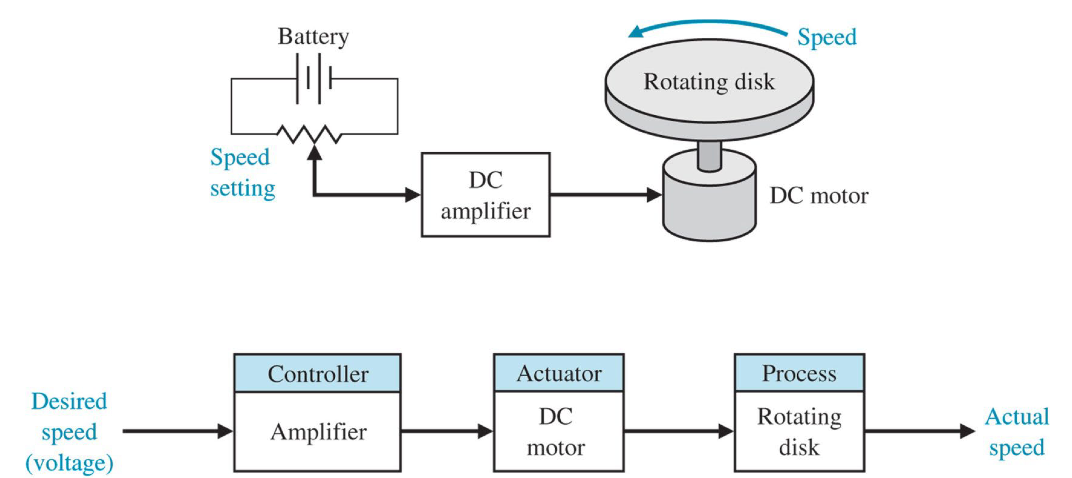
\includegraphics[height=1.35in]{./figures/oploop.png}
    \caption{Open-loop control system.}
    \label{fig:oploop}
  \end{subfigure}
  \hfill
  \begin{subfigure}[t]{0.48\textwidth}
    \centering
    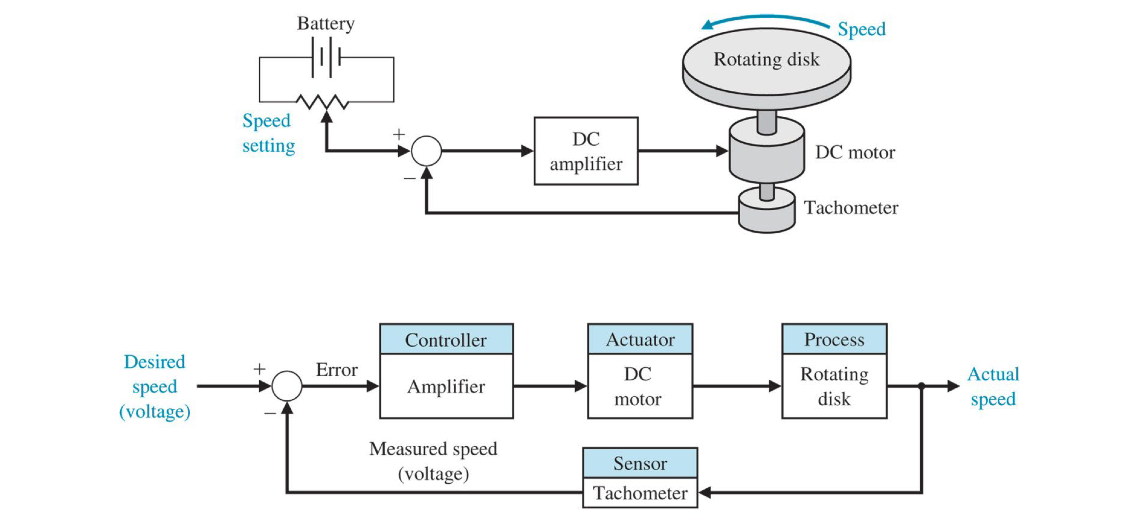
\includegraphics[height=1.35in]{./figures/closloop.png}
    \caption{Closed-loop control system.}
    \label{fig:closloop}
  \end{subfigure}
  \caption{Comparison of an open and closed loop control system.}
\end{figure}

In general an open-loop control system are much simpler than as they do not require any sensors and do not introduce any stability problems on their own.
However, their performance is also rather poor compared to closed-loop systems to match the desired output well.

Closed-loop systems excel in that they do not need human adjustment and are able to respond to disturbance.
These, however, may experience steady-state error or cause stability problems.

\section{Description of the dynamic behavior of physical systems by Differential Equations}
Many different physical systems are governed by differential equations.

\begin{exa}[Spring-Mass-Damper Mechanical system]
  On \Cref{fig:smd} a mass $M$ can move vertically up or down.
  It is connected to a spring with stiffness $k$, a damper with damping/friction coefficient $b$, and an applied external force $r(t)$.

  The acceleration of the mass is related to the net force by Newton's second law:
  \begin{equation*}
    M \ddot{y} = r(t) - b \dot{y} - ky \implies M \ddot{y} + b \dot{y} + ky = r(t)
  .\end{equation*}
\end{exa}

\begin{figure} [ht]
  \centering
  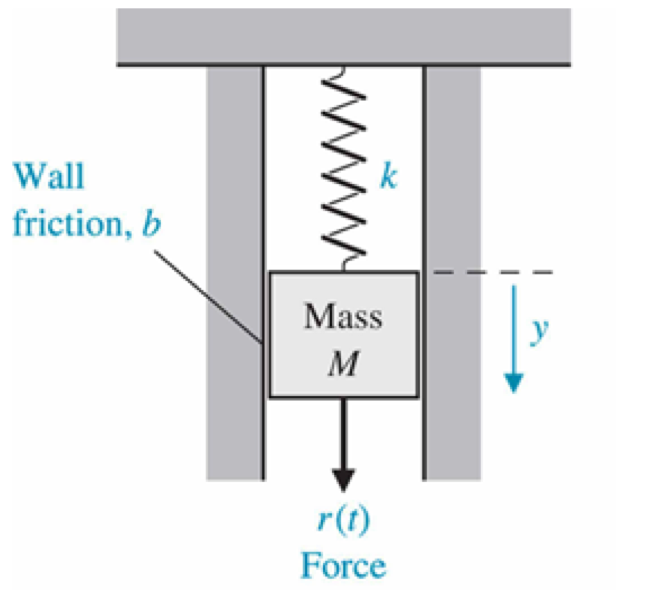
\includegraphics[width=0.4\linewidth]{./figures/smd.png}
  \caption{Spring-mass-damper system.}
  \label{fig:smd}
\end{figure}

\begin{exa}[Resister-inductor-capacitor Circuit Electrical System]
  On \Cref{fig:rlc} a parallel RLC circuit is driven by an input current source $r(t)$ and the output is the voltage $v(t)$ across the branches.
  Here, the resister gives a current proportional to voltage:
  \begin{equation*}
    i_R = \frac{v}{R}
  ,\end{equation*}
  the capacitor has a current of:
  \begin{equation*}
    i_C = C \frac{\mathrm{d}v}{\mathrm{d}t} 
  ,\end{equation*}
  and the voltage-current relation of the inductor is:
  \begin{equation*}
    v = L \frac{\mathrm{d}i_L}{\mathrm{d}t} 
  .\end{equation*}
  
  If we apply Kirchoff's current law at the top node:
  \begin{equation*}
    r(t) = i_R + i_L + i_C
  \end{equation*}
  and then substitute into the branch relations:
  \begin{equation*}
    r(t) = \frac{v}{R} + i_L + C \frac{\mathrm{d}v}{\mathrm{d}t}
  .\end{equation*}
  Taking the time-derivative yields:
  \begin{equation*}
    \frac{\mathrm{d}r}{\mathrm{d}t} = \frac{1}{R} \frac{\mathrm{d}v}{\mathrm{d}t}  + \frac{\mathrm{d}i_L}{\mathrm{d}t}  + C \frac{\mathrm{d}^2 v}{\mathrm{d}t^2} = \frac{1}{R} \frac{\mathrm{d}v}{\mathrm{d}t} + \frac{v}{L} + C \frac{\mathrm{d}^2 v}{\mathrm{d}t^2} 
  .\end{equation*}
  Which can be rearranged to
  \begin{equation*}
    C \frac{\mathrm{d}^2 v}{\mathrm{d}t^2} + \frac{1}{R} \frac{\mathrm{d}v}{\mathrm{d}t}  + \frac{1}{L} v = \frac{\mathrm{d}r(t)}{\mathrm{d}t}  
  .\end{equation*}
  Note that this is analogous to the result from the mass-spring-damper system above.
\end{exa}

\begin{figure} [ht]
  \centering
  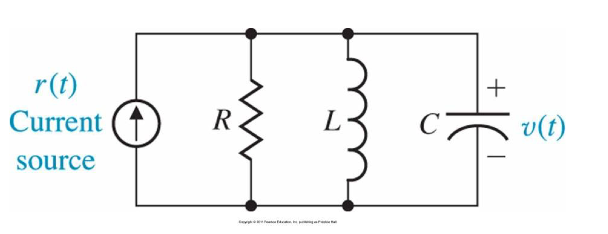
\includegraphics[width=0.6\linewidth]{./figures/rlc.png}
  \caption{Resistor-inductor-capacitor system.}
  \label{fig:rlc}
\end{figure}

In general, many dynamic elements can be broken into inductive storage, capacitive storage, and energy dissipaters.
A table is shown on \Cref{fig:andynel}.

\begin{figure} [ht]
  \centering
  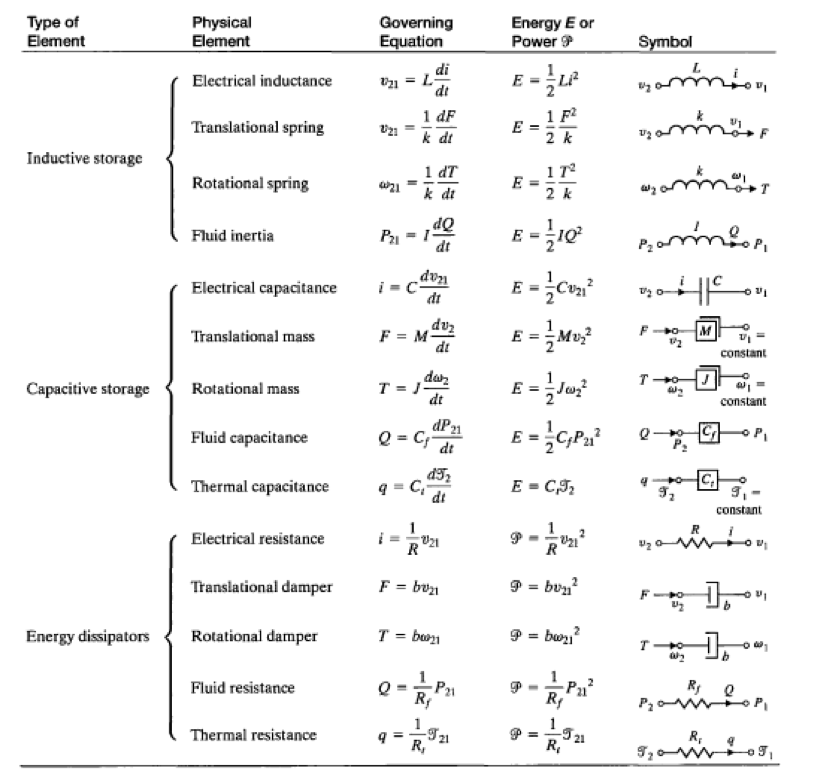
\includegraphics[width=0.6\linewidth]{./figures/andynel.png}
  \caption{Summary of Analogous Dynamic Elements}
  \label{fig:andynel}
\end{figure}

\section{Linear Systems}
A linear system is any system that satisfies superposition.
I.e. if input $u_1$ gives output $y_1$ and input $u_2$ gives output $y_2$, then input $au_1 + b_u2$ gives output $ay_1 + by_2$ for constants $a$ and $b$. 
This means
\begin{equation*}
  m \ddot{y} + b \dot{y} + ky = r(t)
\end{equation*}
is a linear equation as all $y$, $\dot{y}$ and $\ddot{y}$ appear linearly, but
\begin{equation*}
  m \ddot{y} + b \dot{y} + ky^3 = r(t)
\end{equation*}
is nonlinear, due to the $y^3$-term.
An equation like
\begin{equation*}
  \ddot{y} + y \dot{y} = u
\end{equation*}
is also non-linear as $y$ and $\dot{y} $ are multiplied together.

Many non-linear systems can be linearised using Taylor-transforms.


\section{Fundamentals and application of Laplace transforms}
Laplace transforms are used frequently in Control theory to turn differential equations in the time-domain into algebraic equations in the Laplace-domain. 
In general, for a time signal $f(t)$, its Laplace transform is
\begin{equation*}
  F(s) = \mathcal{L} \left\{ f(t) \right\} = \int_{0}^{\infty} f(t) e^{-st} \, \mathrm{d}t 
\end{equation*}
where
\begin{equation*}
  s = \sigma + j\omega
\end{equation*}
is a complex variable.

To go from the Laplace-domain back to the time-domain the inverse Laplace transform, $\mathcal{L}^{-1}$ is used:
\begin{equation*}
  f(t) = \mathcal{L}^{-1} \left\{ F(s) \right\} = \frac{1}{2\pi j} \int_{\sigma - j\infty}^{\sigma + j \infty} F(s) e^{st} \, \mathrm{d}t 
.\end{equation*}
A table of the most important Laplace Transform Pairs is given in \Cref{fig:laptrapair}.

\begin{figure} [ht]
  \centering
  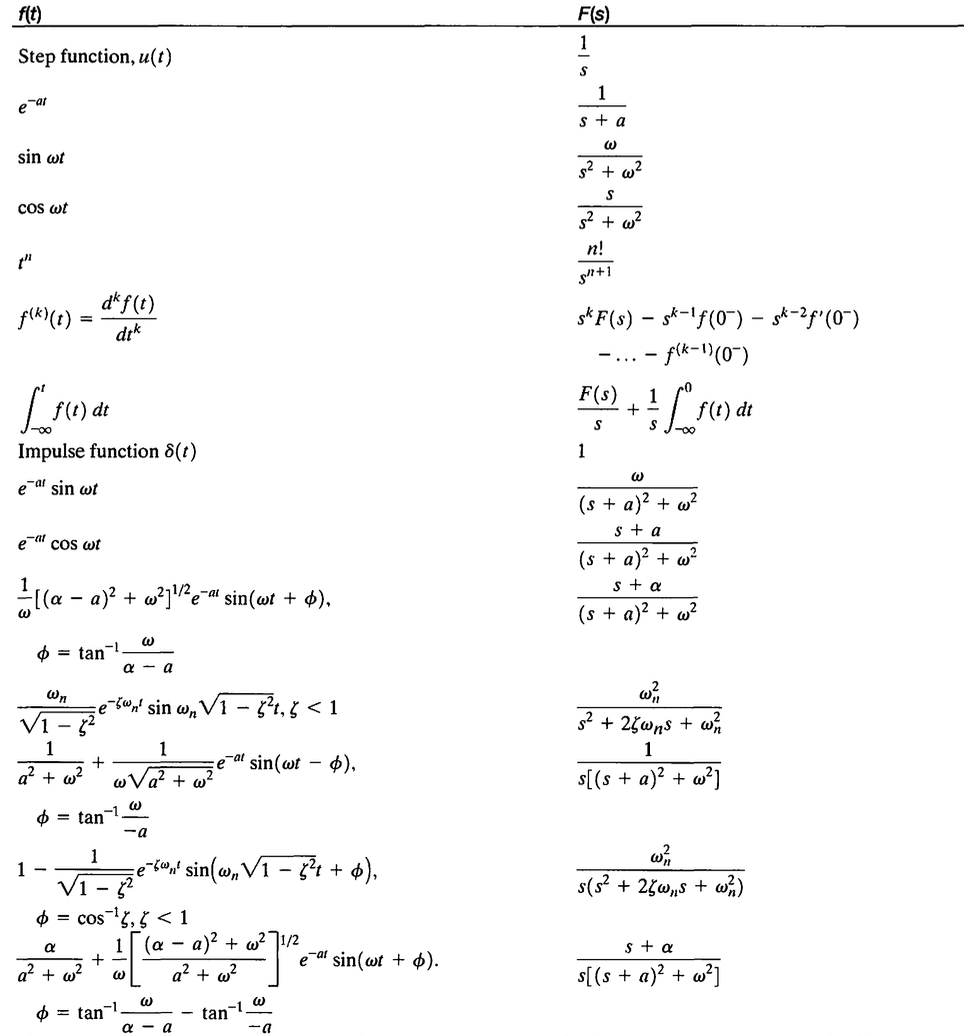
\includegraphics[width=0.9\linewidth]{./figures/laptrapair.png}
  \caption{Important Laplace Transform Pairs}
  \label{fig:laptrapair}
\end{figure}

It is also worth noting that an integral in the time-domain corresponds to division by $s$ in the Laplace-domain:
\begin{equation*}
  \mathcal{L} \left\{ \int_{0}^{\infty} f(t) \, \mathrm{d}t  \right\} = \frac{1}{s} \int_{0}^{\infty} f(t) e^{-st} \, \mathrm{d}t  = \frac{1}{s} F(s)
\end{equation*}
and that a derivative in the time-domain corresponds to multiplication by $s$ in the Laplace-domain
\begin{align*}
  \mathcal{L} \left\{ \frac{\mathrm{d}f(t)}{\mathrm{d}t}  \right\} &= s F(s) - f(0) \\
  \mathcal{L} \left\{ \frac{\mathrm{d}f(t)^2}{\mathrm{d}t^2}  \right\} &= s^2 F(s) - sf(0) - f'(0) \\
  \mathcal{L} \left\{ \frac{\mathrm{d}f(t)^3}{\mathrm{d}t^3} \right\} &= s^3 F(s) - s^2 f(0) - s f'(0) - f''(0) \\
    &\vdots \\
  \mathcal{L} \left\{ \frac{\mathrm{d}f(t)^{n}}{\mathrm{d}t ^{n}}  \right\} &= s^{n} F(s) - s^{n-1} f(0) - s^{n-2} f'(0) - \ldots  - f^{(n-1)}(0)
.\end{align*}

Further, addition/scaling of Laplace transforms follows the relation
\begin{equation*}
  \mathcal{L} \left\{ a f_1(t) \pm bf_2(t) \right\} = aF_1(s) \pm bF_2(s)
,\end{equation*}
convolutions are defined as
\begin{equation*}
  \int_{0}^{t} f_1(t - \tau) f_2(\tau) \, \mathrm{d}\tau = F_1(s) F_2(s)
,\end{equation*}
the initial-value theorem is
\begin{equation*}
  f(0+) = \lim_{s \to \infty} s F(s)
,\end{equation*}
and the final-value theorem is
\begin{equation*}
  \lim_{t \to \infty}f(t) = \lim_{s \to 0} sF(s)
.\end{equation*}

\subsection{Transfer Functions}
A transfer function is often used to describe the dynamics of a system.
These are defined only for linear, stationary (i.e. constant parameter) systems, and may not apply for time-varying systems having one or mare time-varying parameters.
A transfer function does not include any information about the internal structure of the system.
\begin{definition}[Transfer Function]
  A transfer function is defined as the ratio of the Laplace transform of the output variable to the Laplace transform of the input variable, with all initial conditions assumed to be zero.
  I.e. the transfer function $G(s)$ of the Laplace transform $Y(s)$ of the output $y(t)$ and the Laplace transform $R(s)$ of the input $r(t)$ is
  \begin{equation*}
    G(s) = \frac{Y(s)}{R(s)}
  .\end{equation*}
\end{definition}

\begin{exa}[Transfer function of a Mass-spring-damper]
  For a mass-spring-damper such as that on \Cref{fig:smd} we have Newton's second law:
  \begin{equation*}
    M \frac{\mathrm{d}^2 y}{\mathrm{d}t^2} + b \frac{\mathrm{d}y}{\mathrm{d}t} + ky = r(t) 
  .\end{equation*}
  Now, taking the Laplace transform with zero initial conditions:
  \begin{equation*}
    M s^2 Y(s) + bs Y(s) + kY(s) = R(s) \implies Y(s) \left( Ms^2 + bs + k \right) = R(s)
  .\end{equation*}
  So:
  \begin{equation*}
    G(s) = \frac{Y(s)}{R(s)} = \frac{1}{Ms^2 + bs + k}
  .\end{equation*}
\end{exa}

In general for an $n$-th order linear differential equation:
\begin{equation*}
  \frac{\mathrm{d}^{n}y}{\mathrm{d}t^{n}} + q_{n-1} \frac{\mathrm{d}^{n-1}}{\mathrm{d}t ^{n-1}} + \ldots + q_0 y = p_{n-1} \frac{\mathrm{d}^{n-1}r}{\mathrm{d}t ^{n-1}} + p_{n-2} \frac{\mathrm{d}^{n-2} t}{\mathrm{d}t ^{n-2}} + \ldots + p_0 r 
,\end{equation*}
after taking the Laplace transform the transfer function will look like:
\begin{equation*}
  G(s) = \frac{Y(S)}{R(s)} = \frac{p_{n-1} s^{n-1} + p_{n-2} s^{n-2} + \ldots + p_0}{s^{n} + q_{n-1} s^{n-1} + \ldots + q_0} = \frac{p(s)}{q(s)}
.\end{equation*}
So in general, a transfer function is a ratio of two polynomials in $s$.

\subsubsection{Poles and Zeros}
From
\begin{equation*}
  G(s) = \frac{p(s)}{q(s)}
\end{equation*}
we define zeros to be the roots of $p(s) = 0$ and the poles to be the roots of $q(s) = 0$. 

This means that zeros are values of $s$ that make the transfer function become zero.
These change how the system responds to input and affect transient behavior, frequency response, overshoot, etc. 

The poles are more fundamental for system dynamics and determine stability, oscillation, decay rate and speed of responds.
Poles with positive real part cause growth and instability as these lead to positive exponentials $e^{t}$ after taking the inverse Laplace.

\section{Partial Fraction Decomposition}
Given a fraction such as
\begin{equation*}
  \frac{s+1}{(s+2)(s+3)}
\end{equation*}
we wish to split this into a sum of two fractions with simple denominators that we can easily take the inverse Laplace transform of
\begin{equation*}
  \frac{A}{s+2} + \frac{B}{s+3}
\end{equation*}
with some (yet) unknown constants $A$ and $B$. 

To do this we:
\begin{enumerate}
  \item Expand into a term for each factor in the denominator
  \item Recombine the RHS
  \item Equate terms in $s$ and constant terms, and have algebraic equations of the coefficients
  \item Solve algebraic Equations
  \item Each term is in a form so that inverse Laplace transforms can be applied.
\end{enumerate}

Starting with:
\begin{equation*}
  \frac{s+1}{(s+2)(s+3)} = \frac{A}{s+2} + \frac{B}{s+3}
.\end{equation*}
We put the RHS over a common denominator:
\begin{equation*}
  \frac{A}{s+2} + \frac{B}{s+3} = \frac{A(s+3) + B(s+2)}{(s+2)(s+3)}
,\end{equation*}
so now
\begin{equation*}
  \frac{s+1}{(s+2)(s+3)} = \frac{A(s+3) + B(s+2)}{(s+2)(s+3)}
.\end{equation*}
Since the denominators are equal, the numerators must also be equal:
\begin{align*}
  s+1 &= A(s+3) + B(s+2) \\
      &= As + 3A + Bs + 2B \\
      &= (A+B)s + (3A + 2B)
.\end{align*}
From this we see that $A+ B= 1$ and $B = 1-A$, so $A=-1$ and $B = 2$.
I.e.
\begin{equation*}
  \frac{s+1}{(s+2)(s+3)} = - \frac{1}{s+2} + \frac{2}{s+3}
.\end{equation*}
Now, taking the inverse Laplace transform is easy:
\begin{align*}
  \mathcal{L}^{-1} \left\{ \frac{1}{s+a} \right\} &= e^{-at} \\
  \mathcal{L}^{-1} \left\{ \frac{s+1}{(s+2)(s+3)} \right\} &= -e^{-2t} + 2e^{-3t}
.\end{align*}

\begin{exa}[Partial Fraction Decomposition]
  \begin{align*}
    G(s) &= \frac{5s + 3}{(s+1)(s+2)(s+3)} \\
    \frac{5s+3}{(s+1)(s+2)(s+3)} &= \frac{K_{s1}}{s+1} + \frac{K_{s 2}}{s+ 2} + \frac{K_{s 3}}{s + 3} \\
    K_{-1} &= \frac{p(-1)}{(-1+2)(-1+3)} = -1\\
    K_{-2} &= \frac{p(-2)}{(-2+1)(-2+3)} = 7 \\
    K_{-3} &= \frac{p(-3)}{(-3+1)(-3+2)} = -6\\
    \frac{5s + 3}{(s+1) (s+2)(s+3)} &= - \frac{1}{s+1} + \frac{7}{s+2} - \frac{6}{s+3} \\
    G(t) &= -e^{-t} + 7 e^{-2t} - 6 e^{-3t}
  .\end{align*}
\end{exa}

\begin{exa}[Conversion of ODE to Algebraic Equation using Laplace Transforms]
  Given the ODE
  \begin{equation*}
    \frac{\mathrm{d}^2 y}{\mathrm{d}t^2} + 6 \frac{\mathrm{d}y}{\mathrm{d}t} + 8y = 2 \qquad y(0)=y'(0)=0
  \end{equation*}
  we want to find a solution using the Laplace transform to turn the above ODE into an easily-solvable algebraic equation.
  \tcblower
  We start by finding the Laplace transform of each term.
  \begin{align*}
    \frac{\mathrm{d}^2y}{\mathrm{d}t^2} &= s^2 Y(s) - sy(0) - y'(0) \\
    6 \frac{\mathrm{d}y}{\mathrm{d}t} &= 6 \left( sY(s) - y(0) \right) \\
    8y &= 8Y(s) \\
    2 &= \frac{2}{s} \\
    s^2 Y(s) - 0 - 0 + 6 \left( sY(s) - 0 \right) + 8Y(s) &= \frac{2}{s} \\
    s^2 Y(s) + 6sY(s) + 8Y(s) &= \frac{2}{s} \\
    Y(s) \left( s^2 + 6s + 8 \right) &= \frac{2}{s} \\
    Y(s) &= \frac{2}{s \left( s+2 \right) \left( s+4 \right)}
  .\end{align*}
  We have now found the solution in the Laplace-domain.
  To find the corresponding time-domain solution we take the inverse Laplace transform.
  To do this we use Partial Fraction Decomposition:
  \begin{align*}
    \frac{2}{s \left( s+2 \right) \left( s+4 \right)} &= \frac{K_{s 1}}{s} + \frac{K_{s 2}}{s + 2} + \frac{K_{s 3}}{s + 4}\\
    K_{0} &= \frac{2}{2 \cdot 4} = \frac{1}{4} \\
    K_{-2} &= \frac{2}{-2 \cdot 2} = - \frac{1}{2} \\
    K_{-4} &= \frac{2}{-4 \cdot -2} = \frac{1}{4} \\
    \frac{2}{s (s+2)(s+4)} &= \frac{1}{4 s} - \frac{1}{2(s + 2)} + \frac{1}{4(s + 4)}\\
  .\end{align*}
  Now, that a partial fraction decomposition has been made we can easily take the inverse Laplace of the solution as
  \begin{align*}
    g(t) &= \frac{1}{4} - \frac{1}{2} e^{-2t} + \frac{1}{4} e^{-4t} \\
     &= \frac{1}{4} e^{-4 t} \left(e^{2 t}-1\right)^2
  .\end{align*}
\end{exa}

\begin{exa}[In-Class Exercise: Controlling a Laser Printer]
  A laser printer uses a laser beam to print copy rapidly for a computer. The laser is positioned by a control input $r(t)$, so that we have
  \begin{equation*}
    Y(s) = \frac{4(s+50)}{s^2 + 30s + 200}R(s)
  .\end{equation*}
  The input $r(t)$ represents the desired position of the laser beam.
  \begin{enumerate}[label=(\alph*)]
    \item If $r(t)$ is a unit step input find the output $y(t)$.
    \item What is the final value of $y(t)$?
  \end{enumerate}
  \tcblower
  \begin{enumerate}[label=(\alph*)]
    \item   For a unit step $r(t)$, $R(s) = \frac{1}{s}$, so
  \begin{align*}
    Y(s) &= \frac{4(s+50)}{s^2 + 30s + 200} \frac{1}{s} \\
    &= \frac{4(s+50)}{s^3 + 30s^2 + 200s} \\
    &= \frac{4(s+50)}{s (s+10)(s+20)} \\
    \frac{4(s+50)}{s(s+10)(s+20)} &= \frac{K_{0}}{s} + \frac{K_{10}}{s+10} + \frac{K_{20}}{s+20} \\
    K_{0} &= \frac{200}{10 \cdot 20} = 1 \\
    K_{-10} &= \frac{160}{-10 \cdot 10} = - \frac{8}{5} \\
    K_{-20} &= \frac{120}{-20 \cdot -10} = \frac{3}{5} \\
    Y(s) &= \frac{1}{s} - \frac{8}{5(s+10)} + \frac{3}{5(s+20)} \\
    y(t) &= 1 - \frac{8}{5}e^{-10t} + \frac{3}{5} e^{-20t}
  .\end{align*}
  \item We solve:
    \begin{equation*}
      \lim_{t \to \infty} 1 - \frac{8}{5} e^{-10t} + \frac{3}{5} e^{-20t} = 1
    .\end{equation*}
  \end{enumerate}
\end{exa}
